% ================================================================
% Neural Demand Paper — CF Tables (auto-generated)
% N_RUNS = 5
% ================================================================

\begin{table}[htbp]
  \centering
  \caption{Control-Function First-Stage $R^2$ (Hausman Instruments)}
  \label{tab:cf_rsq}
  \begin{tabular}{lccc}
    \toprule
    & \textbf{Aspirin} & \textbf{Acetaminophen} & \textbf{Ibuprofen} \\
    \midrule
    $R^2$ & $0.541$ & $0.585$ & $0.464$ \\
    \bottomrule
  \end{tabular}
  \begin{tablenotes}\small
    \item Hausman mean-price instruments. First-stage OLS of log price on instruments.
  \end{tablenotes}
\end{table}

\begin{table}[htbp]
  \centering
  \caption{Compensating Variation --- CF Decomposition (10\% Aspirin shock)}
  \label{tab:cf_welfare}
  \begin{tabular}{lc}
    \toprule
    \textbf{Model} & \textbf{CV (£ per household)} \\
    \midrule
    LA-AIDS & $-0.2322$ \\
    BLP (IV) & $-0.2212$ \\
    QUAIDS & $-0.2339$ \\
    Series Est. & $-0.2333$ \\
    LDS (Shared) & $-0.2823$ \\
    LDS (GoodSpec) & $-0.2818$ \\
    LDS (Orth) & $-0.2407$ \\
    Neural Demand (static) & $-0.2376 \pm 0.0008$ \\
    Neural Demand (habit) & $-0.2107 \pm 0.0004$ \\
    Neural Demand (CF) & $-0.2261 \pm 0.0004$ \\
    Neural Demand (habit, CF) & $-0.2145 \pm 0.0005$ \\
    \bottomrule
  \end{tabular}
  \begin{tablenotes}\small
    \item CV for 10\% increase in Aspirin price at test-mean prices.
    Values at structural evaluation ($\hat{v}=0$).
  \end{tablenotes}
\end{table}

\begin{figure}[htbp]
  \centering
  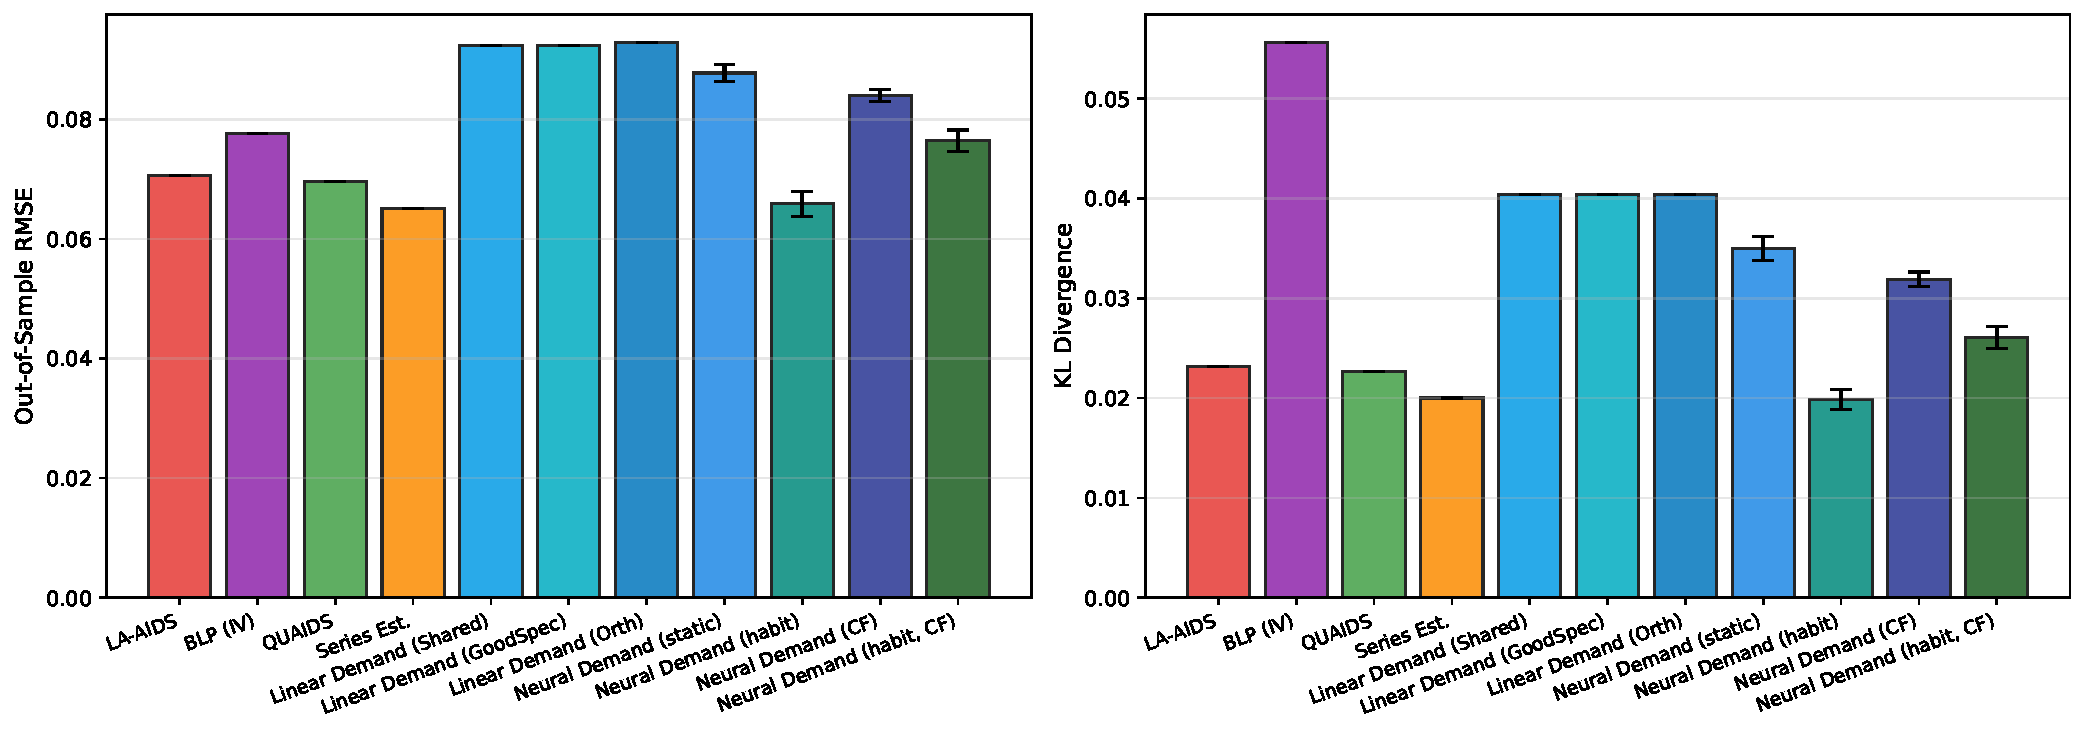
\includegraphics[width=0.85\linewidth]{results/neural_demand/dominicks/figures/fig_cf_accuracy.pdf}
  \caption{CF Correction: RMSE and KL Divergence. Columns show the three-way decomposition: uncorrected, CF-corrected static, and CF-corrected with habit.}
  \label{fig:cf_accuracy}
\end{figure}

\begin{figure}[htbp]
  \centering
  \includegraphics[width=0.85\linewidth]{results/neural_demand/dominicks/figures/fig_cf_demand_curves.pdf}
  \caption{Demand Curves — CF Decomposition. Aspirin budget share as its price varies. CF-corrected curves recover the structural preference component.}
  \label{fig:cf_demand_curves}
\end{figure}

\begin{figure}[htbp]
  \centering
  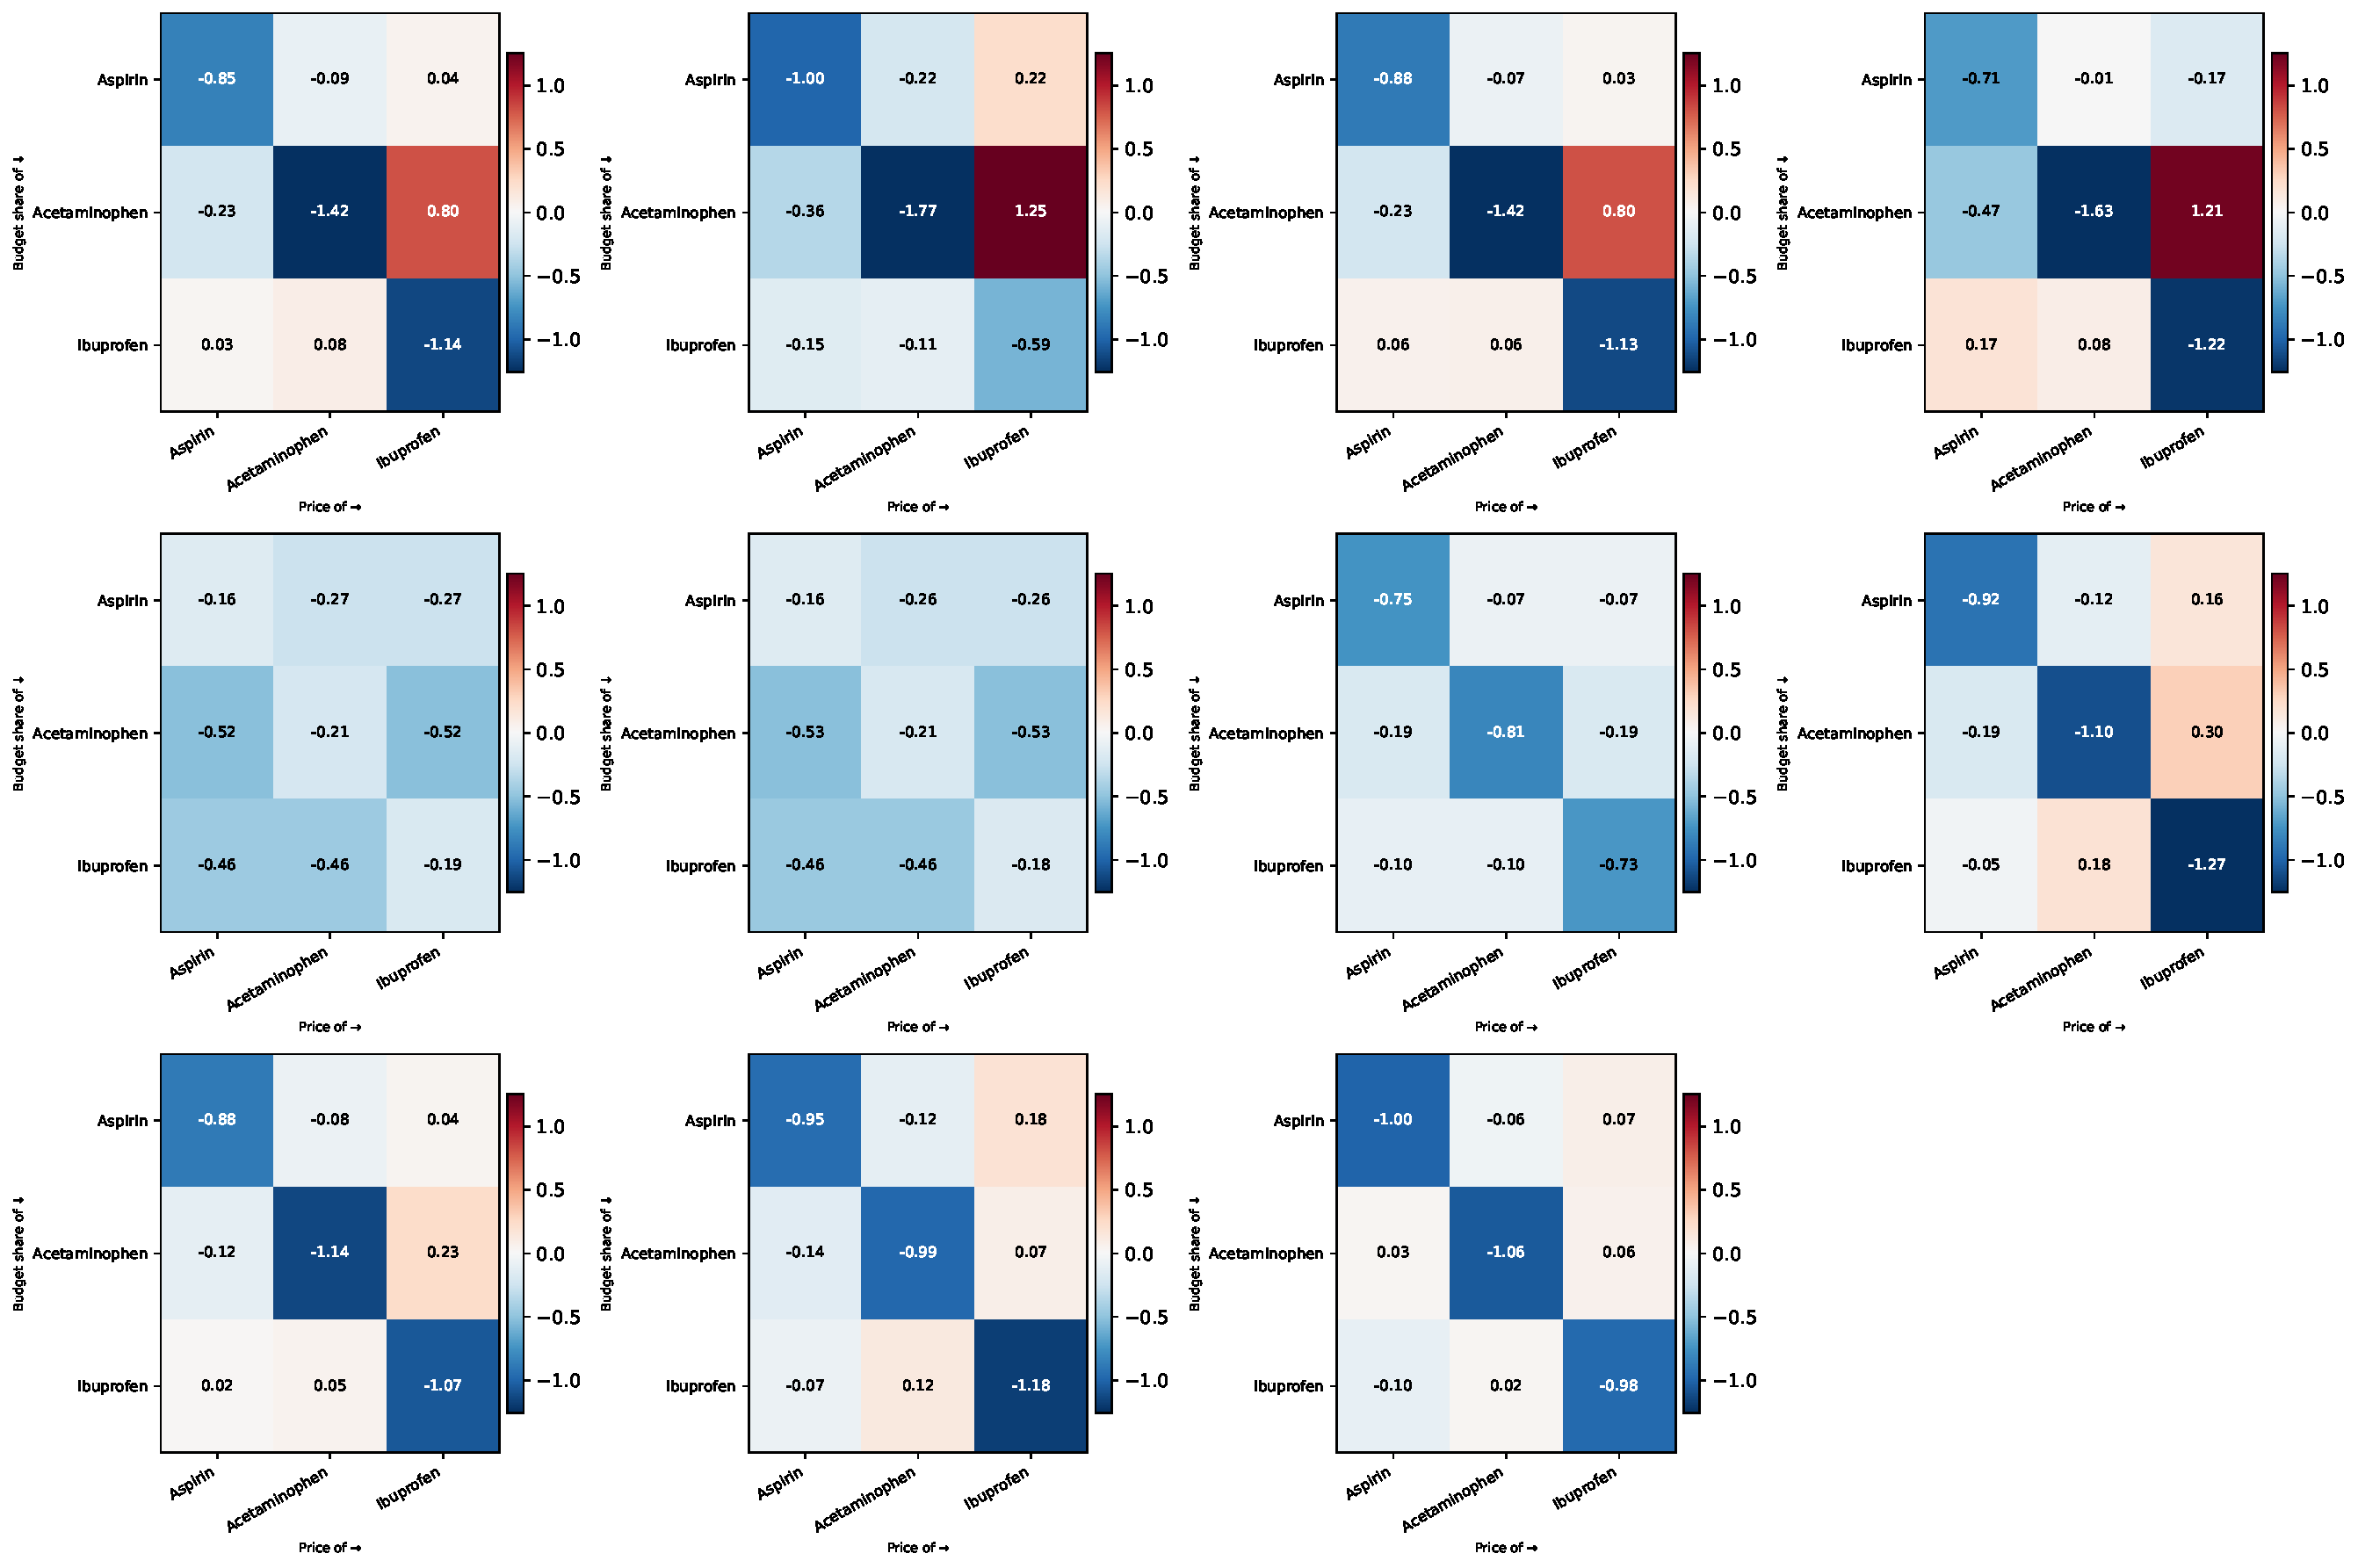
\includegraphics[width=0.85\linewidth]{results/neural_demand/dominicks/figures/fig_cf_elasticity_heatmap.pdf}
  \caption{Own-Price Elasticity Heatmaps for the three CF-decomposition models.}
  \label{fig:cf_elasticity_heatmap}
\end{figure}
